\clearpage
\section{Assessment of the performance of estimators using a simulation study}\label{Simulation}

\subsection{Simulation method}
A simulation study, in which synthetic data with characteristics that are as close as possible to those that may occur in real life, may be used to better understand of  performance of the estimators presented in chapter~\ref{Estimators} in terms of:
\begin{itemize}
	\item The dependence of the precision (the width of the 95\% confidence interval) of the estimates, as a function of sample size, variability in the key process parameters (EF and flow rate) and the strength of the relationship between auxiliary variable and EF
	\item The coverage probability of the 95\% confidence intervals, measured by the proportion of times that the confidence intervals contain the true value of the annual average EF used to generate the synthetic data sets. 
\end{itemize}

An estimator yields valid results only if its associated coverage probability is (close to) 95\%. A good, or efficient, estimator yields, for a given sample size and scenario, a small width of the confidence interval whilst maintaining good coverage probability. If a high precision (small width of confidence interval) is associated with a coverage probability that is too low, then the precision estimate is misleading.

Scenarios are defined by a combination of the following:
\begin{itemize}
	\item The number of laboratory measurements
	\item The correlation (strength of relationship) between the auxiliary variable and the laboratory measurements
	\item The variability in EF, auxiliary variable and flow rate measurements (due to a combination of process variability and measurement errors)
	\item The correlation (strength of relationship) between flow rate and EF, and between flow rate and auxiliary variable
\end{itemize} 

It is assumed that the flow rate and auxiliary variable is monitored continuously, so that the uncertainty regarding for example the average, or weighted average, of the flow rate and auxiliary variable is negligible. At the point of writing this report, only a single auxiliary variable is used in the simulation study. 

Many synthetic data sets are created, each with $4\times24\times365=35040$ triples of measurements $(Y_j,B_j,X_j)$, representing a hypothetical situation in which all variables of interest were monitored every 15 minutes during the entire year. 
The true value of the annual average EF is taken to be:
\begin{equation*}
\mu_{true} = \frac{\Sigma[Y_jB_j]}{\Sigma B_j}.
\end{equation*}
The triples of measurements are drawn from a Multivariate Normal (MVN) distribution:

\begin{equation}\label{DrawMVN}
\begin{bmatrix}
Y \\
X \\
B
\end{bmatrix} \sim
\text{MVN} \left( 
\begin{bmatrix}
\mu_Y \\
\mu_X \\
\mu_B
\end{bmatrix},
\begin{bmatrix}
\sigma_{Y}^2 & \rho_{YX}\sigma_{Y}\sigma_{X} & \rho_{YB}\sigma_{Y}\sigma_{B} \\
\rho_{YX}\sigma_{Y}\sigma_{X} & \sigma_{X}^2 & \rho_{XB}\sigma_{X}\sigma_{B} \\
\rho_{YB}\sigma_{Y}\sigma_{B} & \rho_{XB}\sigma_{X}\sigma_{B} & \sigma_{B}^2 \\
\end{bmatrix}
\right),
\end{equation}
where ($\mu_y$,$\sigma_{Y}^2$), ($\mu_x$,$\sigma_{X}^2$) and ($\mu_B$,$\sigma_{B}^2$) are parameters for the mean and variance of the EF, auxiliary variable and flow rate respectively, to be specified to define a scenario. The parameters $\rho_{YX}$, $\rho_{YB}$ and $\rho_{XB}$ denote the correlation between the pairs of variables. In the simulation study,  $\rho_{YX}$ and $\rho_{YB}$ can be set independently, but $\rho_{XB}$ is set to be $\rho_{XB}=\rho_{YX}*\rho_{YB}$. The mean and variance of the auxiliary variable are of no consequence to the estimates as long as this variable is monitored continuously.

The sampling of the fuel gas flow is simulated by drawing $n$ triples $(y_j,b_j,x_j)$ at random without replacement from the set of $k$ triples $(Y_j,B_j,X_j)$.

An outline of the simulation procedure is given in pseudocode in Algorithm~\ref{sims}.

\RestyleAlgo{boxruled}
\LinesNumbered
\DontPrintSemicolon
\SetKwFor{RepTimes}{repeat}{times}{end}
\begin{algorithm}[h] \label{sims}
	\caption{Simulation study to estimate the relative precision and coverage probability of the estimators.}
	Initialize: Choose values for the sample size $n$, the pairs of values for the mean ad variance of the process parameters  ($\mu_y$,$\sigma_{Y}^2$), ($\mu_x$,$\sigma_{X}^2$) and ($\mu_B$,$\sigma_{B}^2$), and the correlation parameters $\rho_{YX}$ and $\rho_{YB}$. Set $I \gets 0$\;
	\RepTimes{M}{
		Generate a synthetic data set of 35040 triples $(Y_j,B_j,X_j)$ using equation~\ref{DrawMVN}.\;
		Compute the true value $\mu_{true}$.\;
		Generate a synthetic sample data set of $n$ triples $(y_j,b_j,x_j)$ by sampling at random without replacement.\;
		Apply the estimators described in chapter~\ref{Estimators} and store the estimated relative precision in a vector.\;
		\If{$\mu_{true}$ is smaller than the upper bound and larger than the lower bound of the 95\% confidence interval}{$I \gets I + 1$}
	}
	Rank the vector of size $M$ with precisions from smallest to largest and take the 2.5 and 97.5 percentiles as estimates of the range of values that the relative precision could take under the defined scenario. The coverage probability $C$ (expressed as a percentage) is given by $C=100 I/M$.
\end{algorithm}

The reliability of the coverage probability $C$ depends on the number of simulations $M$. To assess the uncertainty in the coverage probability due to small number of simulations, a 95\% confidence interval is computed based on the 2.5 and 97.5 percentiles of the Beta distribution: $\text{Beta}(I,M-I)$. 

\subsection{web-App to explore the expected precision of estimates for different sccenarios}\label{webApp}

A simple web-App has been created which allows the user to specify the scenario in terms of the key parameters of interest (see a screen shot of the web-App in figure~\ref{fig:App}):
\begin{itemize}
	\item The sample size $n$.
	\item The mean and standard deviation (defining process variability) of the EF, $\mu_{Y}$ and $\sigma_Y$.
	\item The mean and standard deviation (defining process variability) of the flow rate, $\mu_{B}$ and $\sigma_B$.
	\item The correlation between the auxiliary variable and the EF, $\rho_{XY}$.
	\item The correlation between the flow rate and the EF, $\rho_{YB}$.
\end{itemize}

the use must choose values for these parameters so that synthetic data sets are created that closely resemble the real-life situations.

Additionally, the following must be specified:
\begin{itemize}
	\item The number of simulations (synthetic data sets). The larger the number of simulations, the more precise the estimates of the performance of the estimators will be. For the relative precision, 500 simulations is typically sufficient. For a good estimate of coverage probability, typiclly at least 1000 simulations are required.
	\item A tick box to indicate whether or not Bootstrap estimators should be included. This is computer intensive, and it may take several minutes for the results to be generated.
	\item The number of simulations in the Bootstrap. For a reasonable assessment of the performance of the Bootstrap, at least 1000 simulations are required. The larger the number of Bootstrap simulations and synthetic data sets, the longer it will take for the results to be generated.
\end{itemize}

\begin{figure}[h]
	\centering
	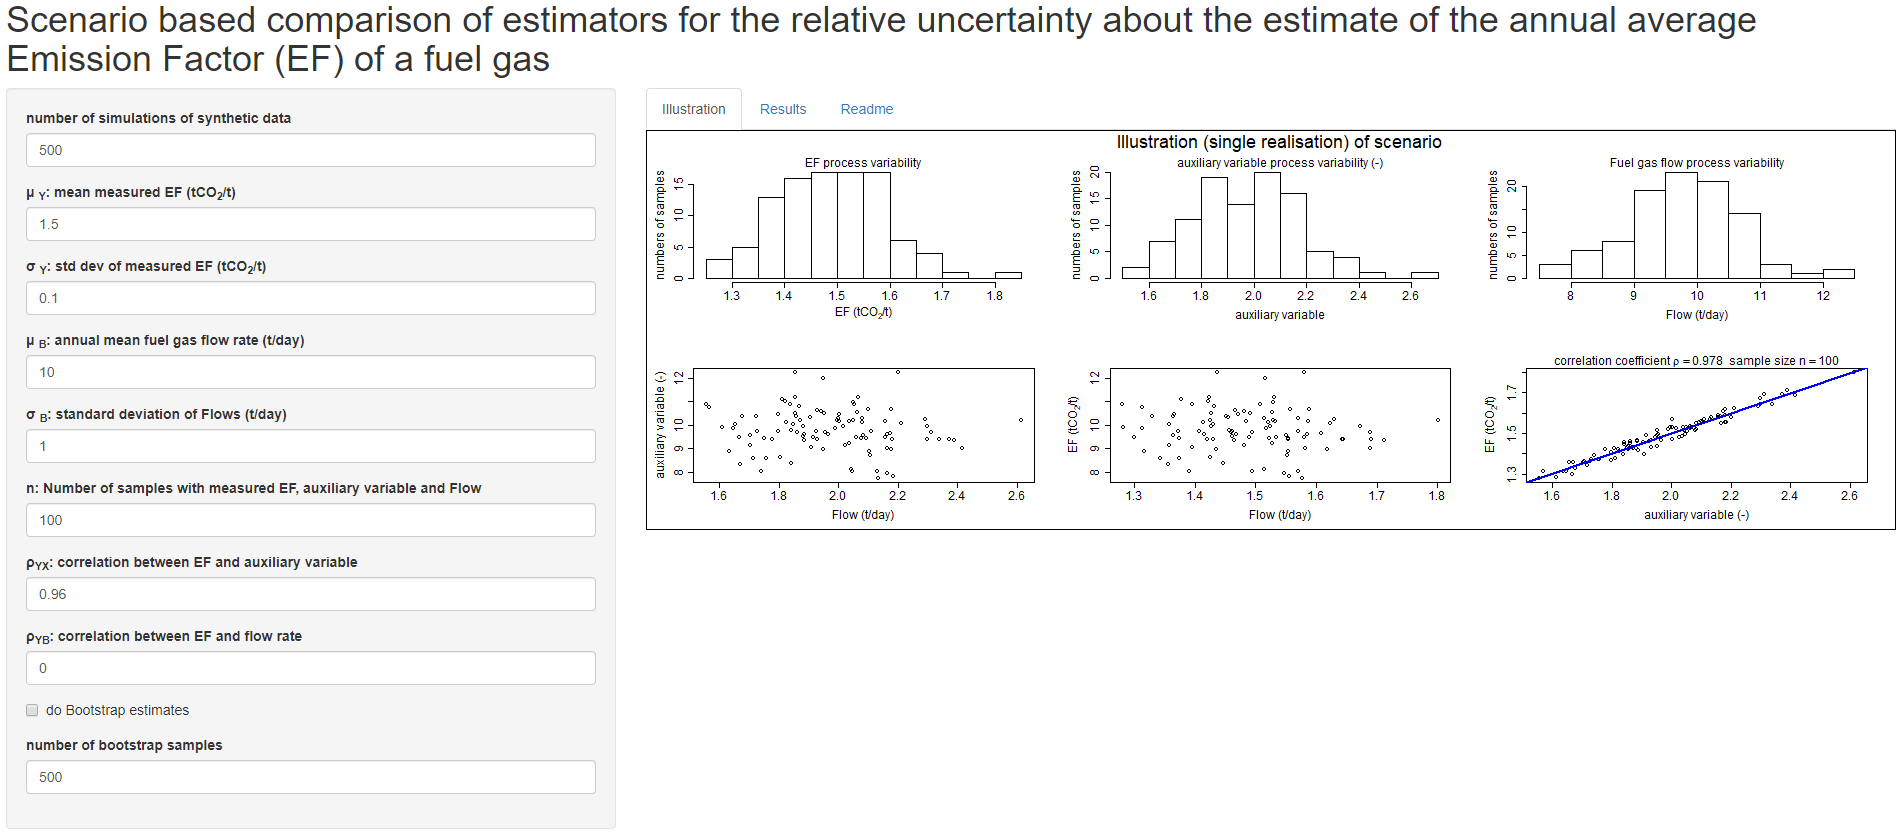
\includegraphics[width=\textwidth]{graphs/AppCapture.PNG}
	\caption{Screen shot of the web-App. On the left are the inputs that define the scenario as well as the number of required simulations. On the right are a number of graphs that illustrate, for a single synthetic data set, what the synthetic data look like. }
	\label{fig:App}
\end{figure}

An illustration of the results of the web-App, for a given scenario with $n=100$ and $\rho_{YX}=0.94$ is given in figure~\ref{fig:AppResults}. For this particular scenario, the estimators without auxiliary variable yield relative uncertainty estimates that are between 2.18\% and 3\%, well above the target set by the NEA of 0.5\%. The corresponding coverage probability is on target: close to 95\%. There is good agreement between the  Bootstrap (section~\ref{SRSBoot}) and Simple Random Sample (SRS; section~\ref{SRS}) estimators. The estimators with auxiliary variables (sections~\ref{AuxBoot},\ref{AuxCochran} and \ref{AuxVZ} all agree well in terms of both relative uncertainty and coverage, and yield uncertainty estimates in the range 0.62\% - 0.85\%, somewhat above the target set by the NEA. 

\begin{figure}[h]
	\centering
	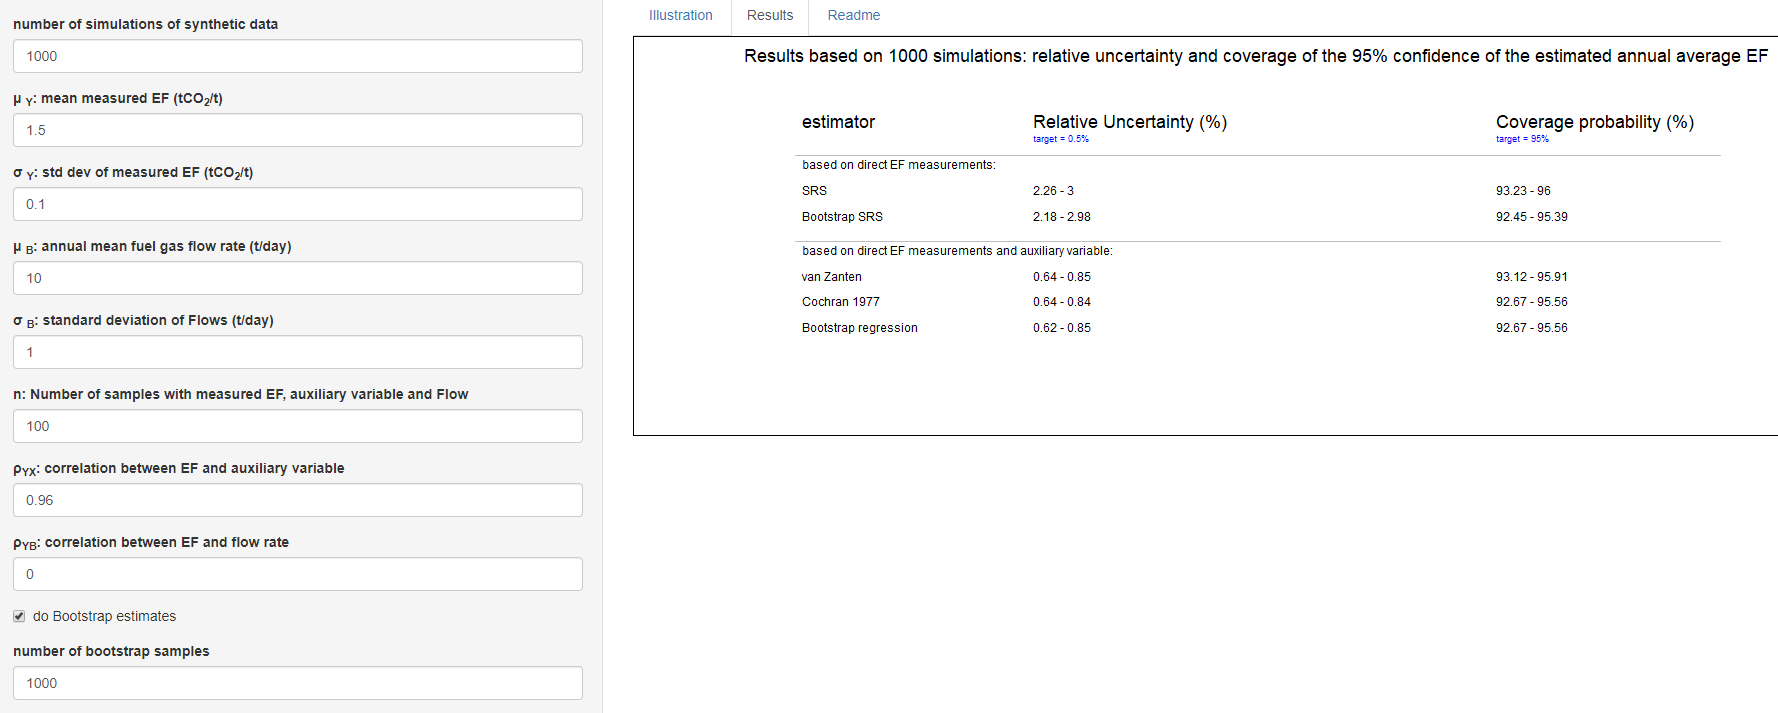
\includegraphics[width=\textwidth]{graphs/ResultsCapture.PNG}
	\caption{Screen shot of the web-App, with results. On the left are the inputs that define the scenario as well as the number of required simulations. On the right are the results in terms of the relative precisions and coverage probabilities. Note that these results took approximately 20 minutes to be generated. }
	\label{fig:AppResults}
\end{figure}


Another illustration of the results of the web-App, for a given scenario with $n=150$ and $\rho_{YX}=0.97$ is given in figure~\ref{fig:AppResults2}. For this particular scenario, the estimators with auxiliary variables (sections~\ref{AuxBoot},\ref{AuxCochran} and \ref{AuxVZ} all agree well in terms of both relative uncertainty and coverage, and yield uncertainty estimates in the range 0.46\% - 0.59\%; depending on chance the esitmate may come in just below or just above the target set by the NEA. 
\begin{figure}[h]
	\centering
	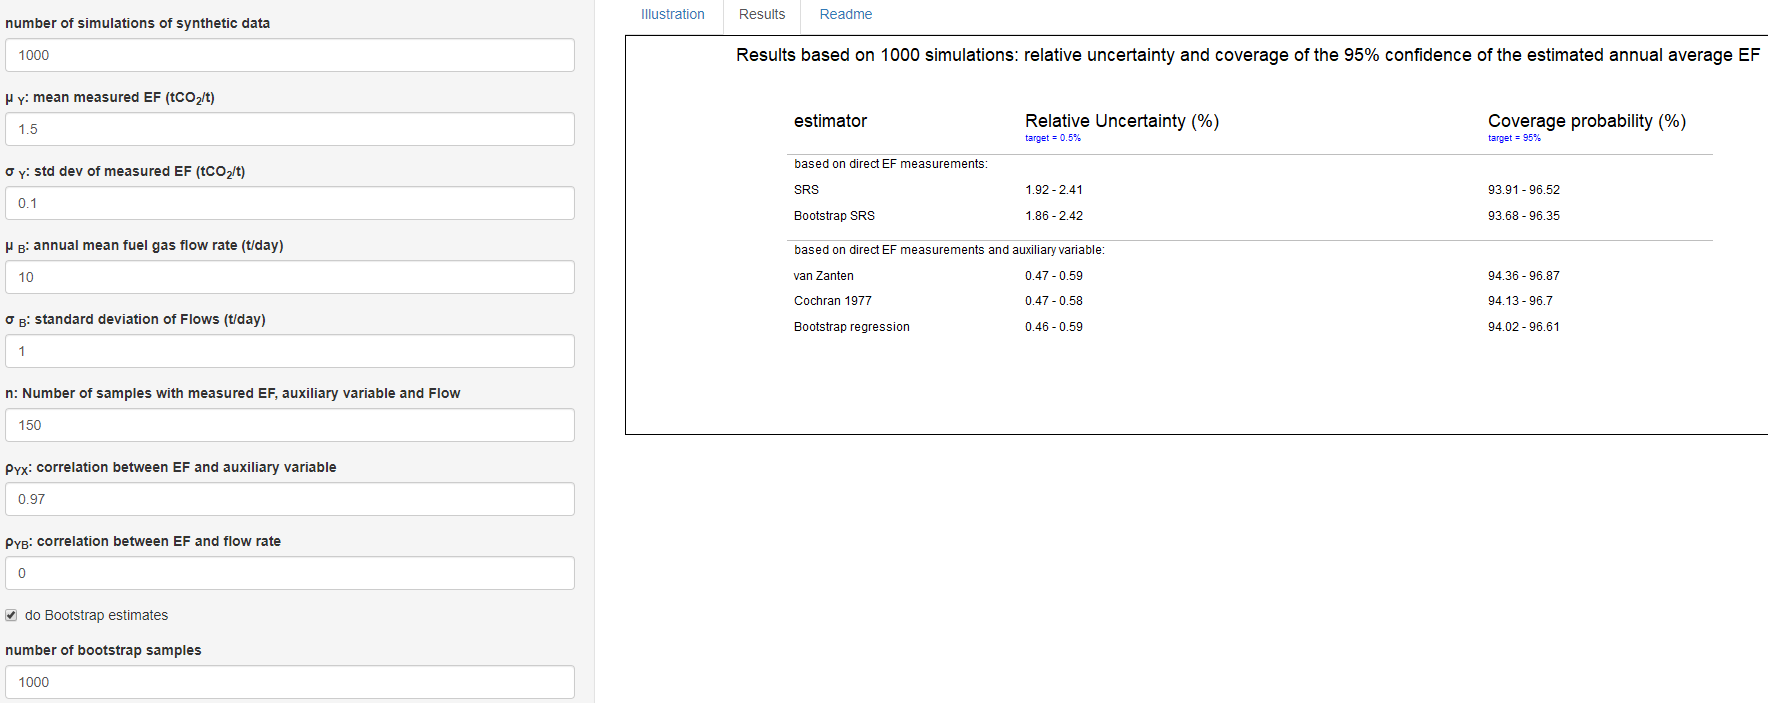
\includegraphics[width=\textwidth]{graphs/ResultsCapture2.PNG}
	\caption{Screen shot of the web-App, with results. On the left are the inputs that define the scenario as well as the number of required simulations. On the right are the results in terms of the relative precisions and coverage probabilities. Note that these results took approximately 20 minutes to be generated. }
	\label{fig:AppResults2}
\end{figure}
